\section{A Case Study: VLIW Hardware/Software Design Space}
\secL{ee}
Since our main focus is the embedded system design, we apply PS to a related case study.
\subsection{Motivation}
In order to evaluate the behavior of the proposed approach
we use a parameterized Very Long Instruction
Word (VLIW) architecture~\cite{kathail_tr00} as testbed. The philosophy
behind a VLIW system makes this a natural choice for several reasons:
\begin{itemize}
\item \emph{Multi-Objective trade-offs}: VLIW architectures allow designers
to trade between power, energy and performances objectives, resulting
in extended Pareto sets which are an ideal ground for our testing
purposes focused on parameter-space representation
\item \emph{Compiler awareness}: code scheduling for the execution of
applications is statically obtained by the compiler which
performs code transformations ``being aware'' of the underlying hardware
configuration.  This tight hardware/software dependence makes the
VLIW scenario perfectly suitable for investigating hardly predictable
parameter interactions.
\end{itemize}

\subsection{Parameter Space}
In general, system parameters can be classified in three main categories:
\emph{processor}, \emph{memory sub-system} and \emph{compiler}. 
The first is directly related to the VLIW core and includes the size
of the register files and the number of functional
units of each type. In particular, five different types of register
files are supported:
GPR (32-bit registers for integers), FPR (64-bit registers for
floating point values) PR (1-bit registers used to store the Boolean
values of predicated instructions), BTR (64-bit registers containing
information about possible future branches) and CR (32-bit control
registers containing information about the internal state of the
processor). The functional units involved are: \emph{Integer units},
\emph{floating point units}, \emph{memory units} (associated with
load/store operations) and \emph{branch units} (associated with branch
operations). With respect to the memory sub-system, the parameters
include \emph{size}, \emph{associativity} and
\emph{block size} for each of the three caches: First-level data cache
(L1D), first-level instruction cache (L1I) and second-level unified
cache (L2U).

Next, a set of the most impacting code compilation parameters has been
selected and included in the configuration space:
\begin{itemize}
\item \emph{tcc\_region}: Specifies the scope of action of the compiler and the type
of code transformation involved (basic block, super block and hyper
block) 
\item \emph {max\_unroll\_allowed}: The number of unroll iterations allowed
\item \emph{regroup\_only}: Avoids inlining 
\item \emph{do\_classic\_opti}: A set of classical optimization, not VLIW related,
such as common expression removal and loop unrolling
\item \emph{do\_prepass\_scalar\_scheduling}: Performs a schedule before
forming regions 
\item \emph{do\_postpass\_scalar\_scheduling}: Performs a schedule after the region formation 
\item \emph{do\_modulo\_scheduling}: Modular scheduling of loop code
\item \emph{memvr\_profiled}: Performs a memory-dependencies profiling 
\end{itemize}

As regards the class of benchmark being considered, a set applications representative of some common
frequently running code kernels has been selected. Table~\ref{tab:bench} shows the set of applications
along with a brief description.
% IEEE table style
%\begin{table}
%	\centering
%	\caption{Benchmarks}
%	\label{tab:bench}
%	\begin{tabular}{ll}
%	\hline
%	\multicolumn{1}{c}{Benchmark} & \multicolumn{1}{c}{Application} \\
%	\hline
%	Alloca\_test & Memory array allocation test \\
%	Bmm & Matrices multiplication and elements sum \\
%	Fir\_int & Finite impulse response \\
%	Mm & Floating point matrices multiplication \\
%	Sha256 & Cryptocurrency header Hashing \\
%	Wave & Wavefront computation \\
%	\hline
%	\end{tabular}
%\end{table}

% ACM table style
\begin{table}
	\tbl{Benchmarks\label{tab:bench}}{
	\begin{tabular}{ll}
	\hline
	\multicolumn{1}{c}{Benchmark} & \multicolumn{1}{c}{Application} \\
	\hline
	Alloca\_test & Memory array allocation test \\
	Bmm & Matrices multiplication and elements sum \\
	Fir\_int & Finite impulse response \\
	Mm & Floating point matrices multiplication \\
	Sha256 & Cryptocurrency header Hashing \\
	Wave & Wavefront computation \\
	\hline
	\end{tabular}}
\end{table}


\subsection{Terms of comparison}

The results presented in the next section compare PS with one widely
adopted Multi-objective Genetic Algorithm
(MOGA)~\cite{knowles_techrep06}. To the best of our knowledge, genetic
approaches in general still represent the best compromise between
efficiency (i.e. time required for exploration) and accuracy of the
reported Pareto Sets.  Note that, for the reasons described above,
mono-objective approaches have been explicitly excluded from this
analysis.  We also exclude other approaches (e.g.  dependency
based~\cite{givargis_tvlsi02}) that make use of some a-priori
knowledge about the role and meaning of each parameter, since our aim
is evaluate the capacity of focusing on interesting parameter regions
without any external judgement or help based on heuristics.  Finally,
it should be pointed out that in this introductory work we will
explicitly use the \emph{SPEA}~\cite{zitzler_eurogen01} variant of
MOGA, remanding to works like~\cite{zitzler_ec00}~\cite{zitzler_tec03}
for a detailed analysis on how it differs from other genetic approaches
and what could be expected from similar multi-objective strategies.


%------------------------------------------------------------------------------
\subsection{Evaluation campaign}
In order to obtain the results presented in this section, we implemented our exploration strategy in Epic Explorer~\cite{ascia2003epic}, an open source framework for the design space explora=tion of embedded systems. \comment{[TODO DAV]: continuare descrivendo un po' il workflow. The reader can refer to~\cite{ascia2003epic} for more details about the estimation models of the power dissipation and execution time. Scrivere che it is possible to run benchmarks }. 

%------------------------------------------------------------------------------

\subsection{Evaluation metrics}
In order to evaluate the Paretos from a quantitative point-of-view we
will consider two metrics, namely, the \emph{variation range} and the
\emph{average normalised absolute dispersion error}. Both of them permit to quantify the extent of the Pareto front that is an important factor to consider when evaluating the quality of a Pareto front. Indeed, authors in \cite{zitzler_ec00,weise2012evolutionary} carefully observe that an exploration algorithm should preferably provide Pareto fronts whose objective function range is large. Following the terminology of~\cite{weise2012evolutionary}, a \emph{uniform convergence} should be guaranteed.
Such Pareto fronts permit to investigate in a broader way the potentials of the designed device. This is important, in general, since if only a narrow portion of the Pareto front is provided due to non-uniform convergence, the decision maker may neglect some important options~\cite{weise2012evolutionary}. Having a narrow Pareto front becomes essential, in particular, when designing a device that may be required to work in different operational conditions, for example with stringent execution time constraints and less strict power dissipation ones or, on the contrary, with low power requirements and tolerance to high execution time.

For a given objective, the \emph{variation range} represents the ratio between the maximum and the minimum value observed for that objective.
\comment{AA: Per rappresentare l'extent del Pereto front, forse sarebbe meglio evitare di usare il variation range, per come l'hai definito tu, e usare la funzione M3 di \cite{zitzler_ec00}, Sec.5 ``Metrics of performance'', che mi pare rappresenti la stessa cosa, concettualmente. Questo ci permette di essere meno attaccabili (del tipo ``non te la prendere con noi, prenditela con Zitzler (che e' citato 3064 volte!) se non capisci l'utilita' della metrica'').}


The average \emph{normalised absolute dispersion error} measures
the average absolute difference between the distribution of points in
the objective space and an ideal distribution in which the points are
uniformly distributed over the objective space. 
Formally, let $O$ be
the image, in the objective space, of the configurations visited by
the design space exploration. The generic element of $O$ (\ie, a
solution) is a pair $(p,t)$ where $p$ and $t$ are the average power
and execution time, respectively. The two-dimensional objective space
is then partitioned by a $M_x \times M_y$ mesh. For each tile $T_i,
\ i=1, 2, \ldots, M_xM_y$ of the mesh, let $N_i$ be the number
of points in $O$ which fall in $T_i$. The average absolute error, $E_i$, for
$T_i$ is the absolute value of the difference between $N_i$ and the
ideal number of solutions, $\overline{N}$, which should fall in $T_i$
in case of uniform distribution. Such $\overline{N}$ can be simply
computed as the ratio between the cardinality of $O$ and the number of
tiles. Thus,
\[ E_i = |N_i - \overline{N}|, \]
where $\overline{N} = |O| / (M_x M_y)$. The average
normalised absolute dispersion error ($ANADE$) is the average of $E_i$
normalised to the maximum absolute error $E_{max}$:
\[ ANADE = \frac{\sum_{i=1}^{M_xM_y} E_i/(M_xM_y)}{E_{max}}, \]
where $E_{max}$ can be computed as the average absolute error in the worst
case in which all the solutions fall in a single tile:
\[ E_{max} = \frac{(M_x M_y - 1) \overline{N} + |\overline{N} -
    |O|| }{M_x M_y}. \] 

\subsection{Impact of the algorithm parameters}
\secL{parameter_impact}
\comment{IMPACT OF $K$. Si potrebbero presentare un plot in cui il numero totale di simulazioni e' fissato e vengono eseguiti diversi run dell'algoritmo con diversi valori di K. Per ogni run, il pareto set e' rappresentato nel plot, sottoforma di una curva diversa. Mi aspetterei che tutte le curve siano molto simili. Per ciascun run, il valore di variation range e average absolute dispersion error sono riportati. Mi aspetto valori simili, il che confermerebbe che la diversity nel nostro algoritmo non dipende da $K$. Ne vale la pena rifare questi run? Ci vuole troppo tempo?} 

\comment{Si potrebbe mettere un plot con nelle ascisse l'era e nelle ordinate il numero di split avvenuti in quell'era. Si potrebbero disegnare diverse curve, una per ogni valore di alpha, per far vedere che il numero di split e' piu' alto q. Recommended values are close to 1, as results in \secR{ee} confirm. Using different values, if sufficiently close to 1, does not have a considerable impact on the resulting Pareto front approximation. Ne vale la pena rifare questi run? Ci vuole troppo tempo?}

\subsection{Results}

\figR{pareto_fronts_100} and \figR{pareto_fronts_500} show the resulting Pareto fronts for two
different scenarios of 100 and 500 simulations budget. \comment{AA: per curiosita': quando facevi piu' run, PS andava ancora peggio rispetto a GA?} When possible,
similar algorithm parameters have been adopted. In particular a
population size of 30 has been chosen for the genetic approach (GA), corresponding to the
same value for the $K$ of PS. \comment{AA: che valore di $alpha$ hai usato?} The number of generations (or era)
has been chosen so that the only the given amount of simulations is
actually performed. Thus, when accounting these simulations only unique simulations
has been considered, removing repetitions and unfeasible
configurations.

% IEEE table style
%\begin{table}
%  \centering
%  \begin{tabular}{ccc}
%    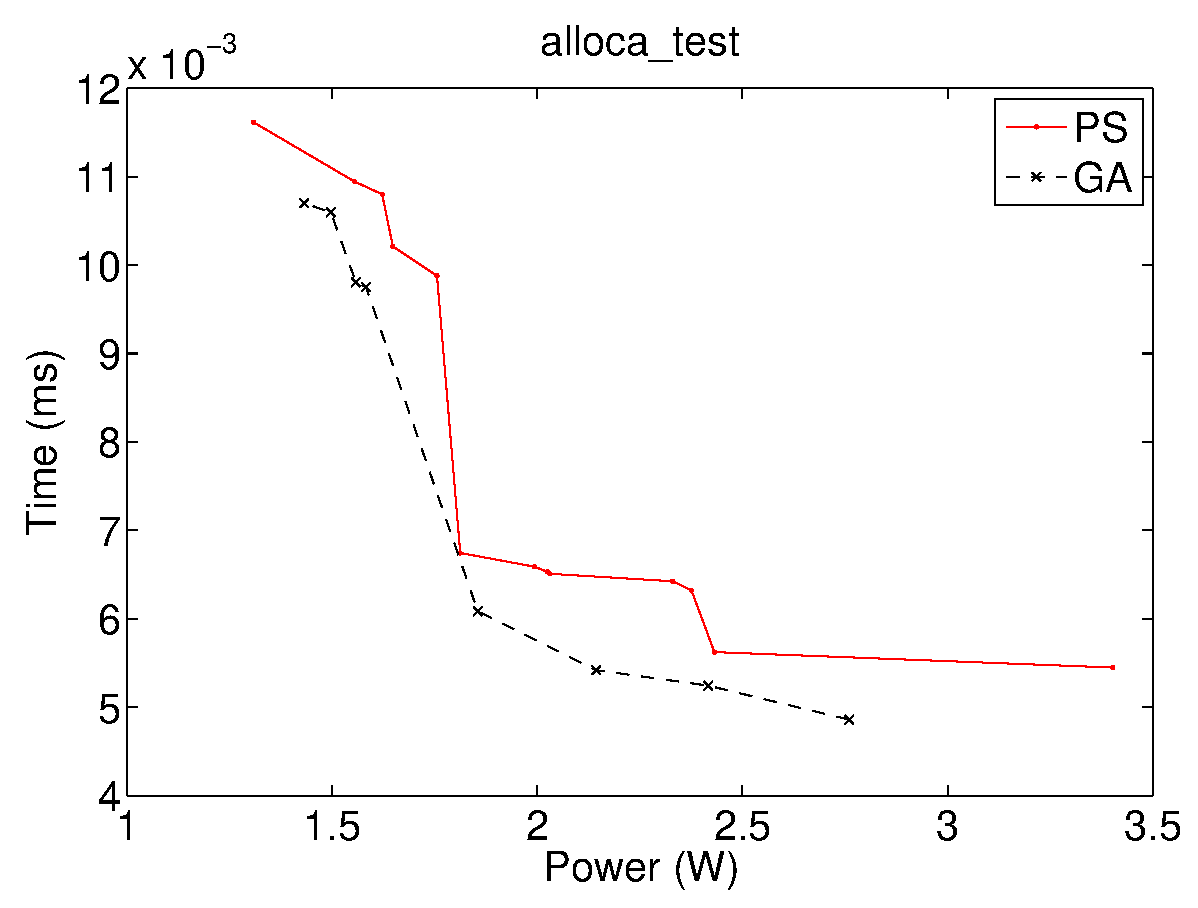
\includegraphics[width=0.30\textwidth]{pictures/alloca_100.eps} &
%    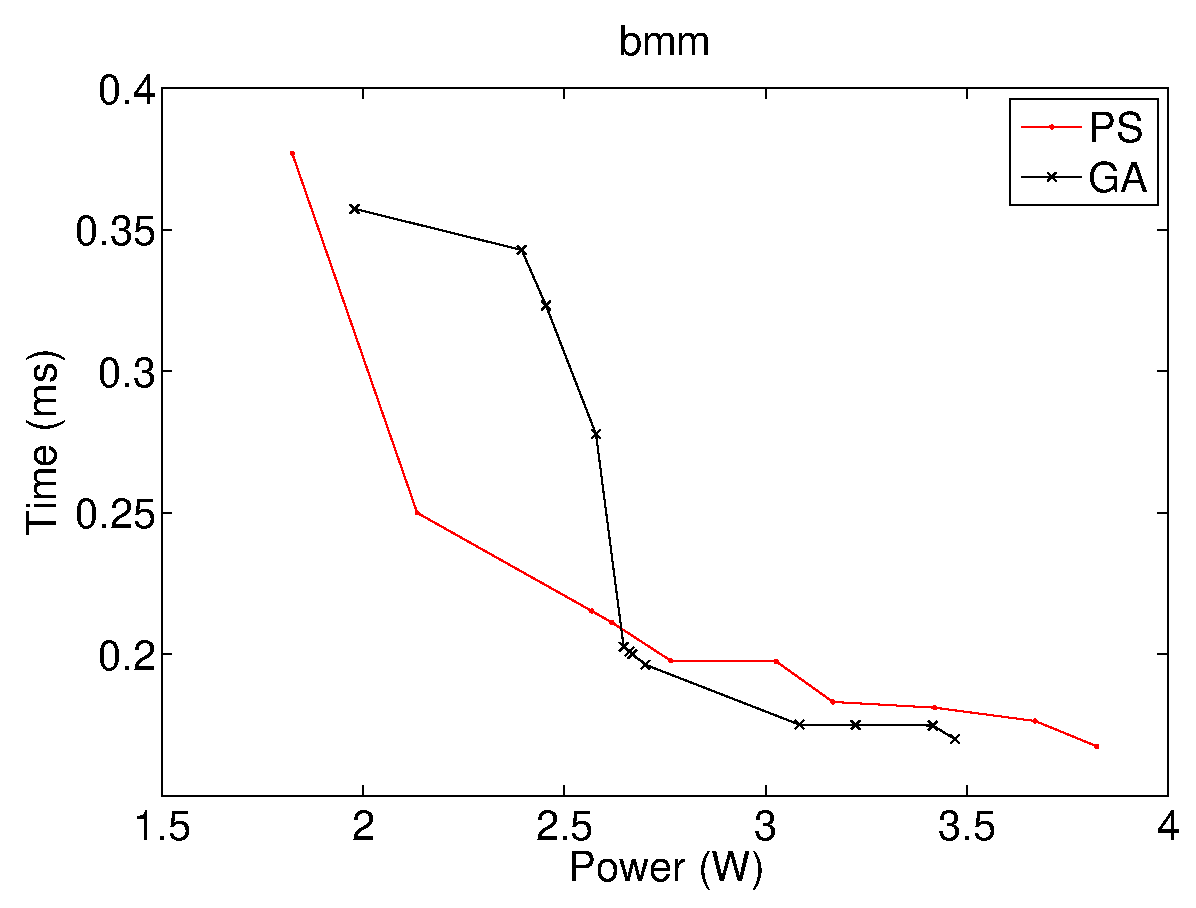
\includegraphics[width=0.30\textwidth]{pictures/bmm_100.eps} & 
%    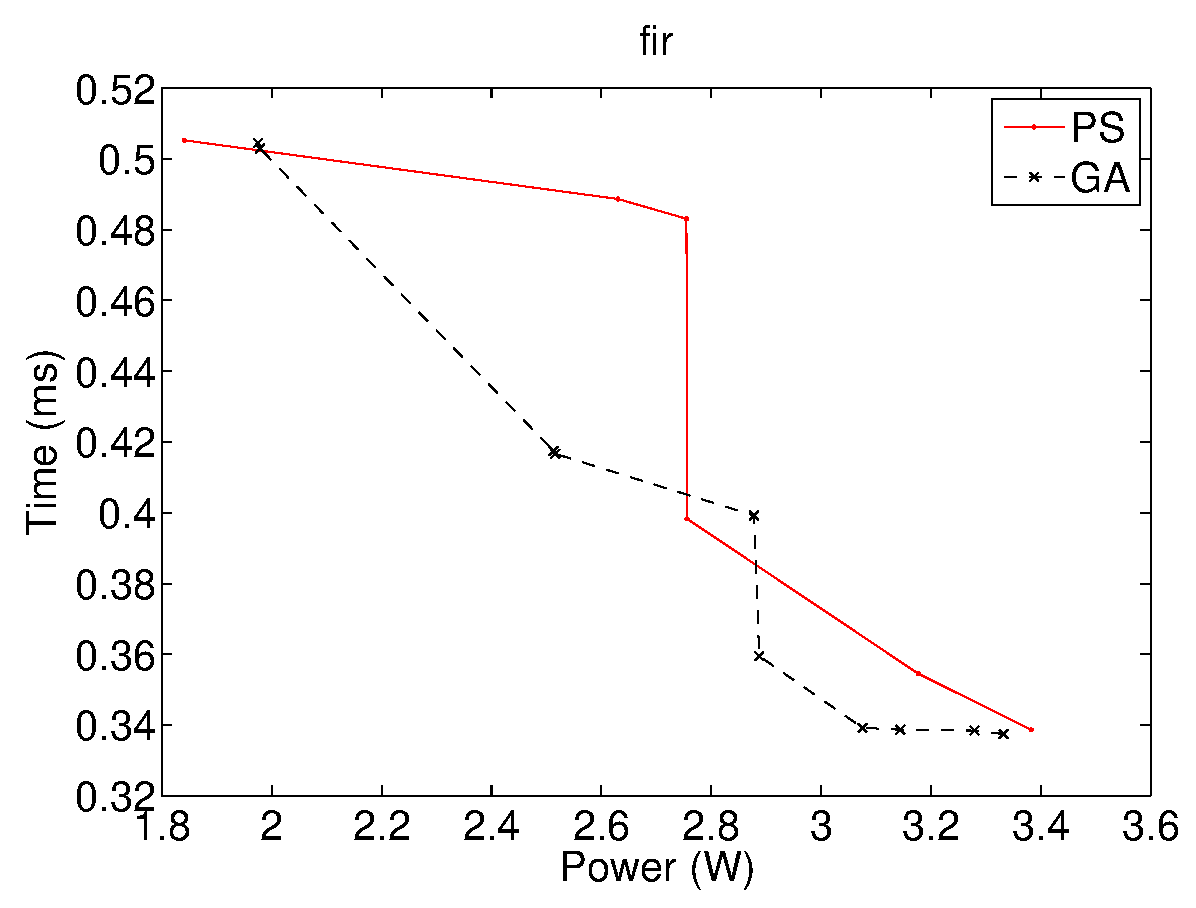
\includegraphics[width=0.30\textwidth]{pictures/fir_int100.eps} \\
%    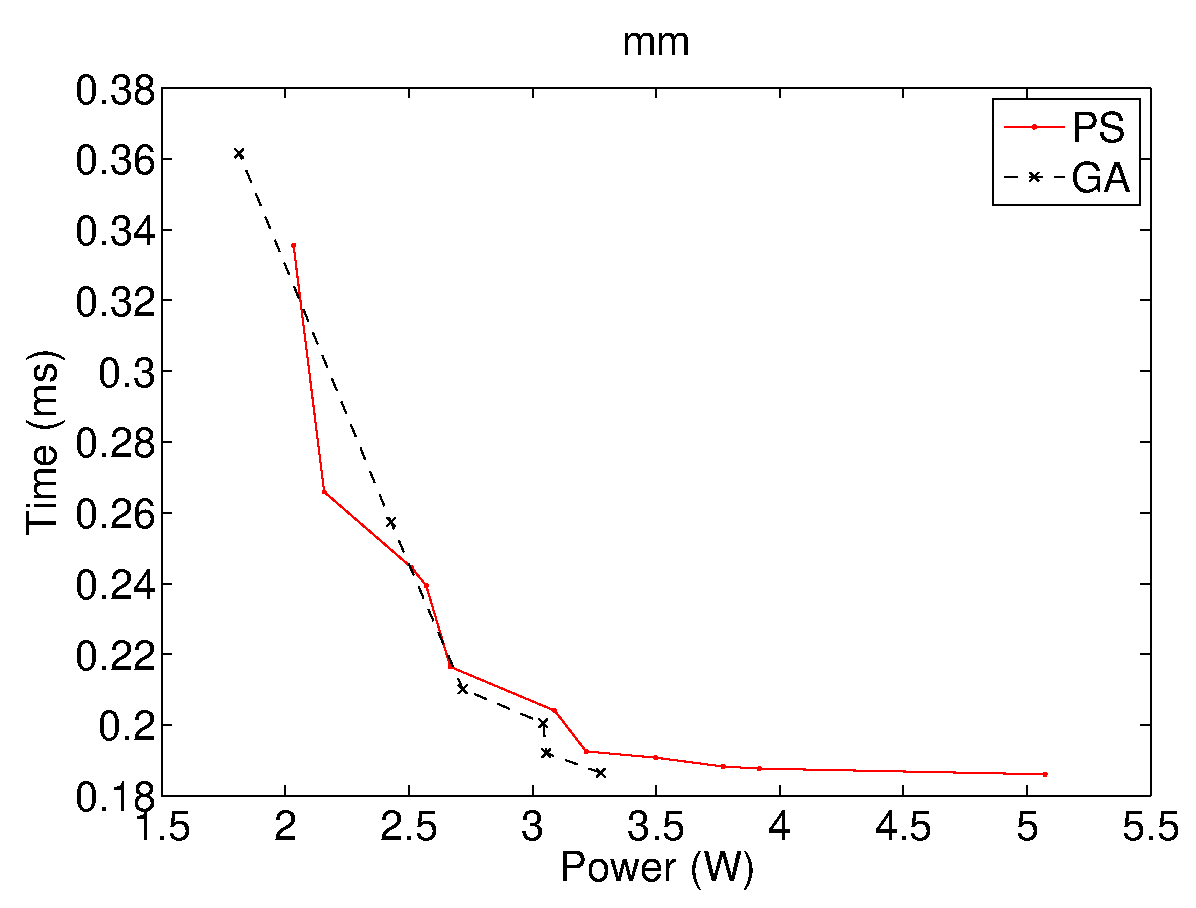
\includegraphics[width=0.30\textwidth]{pictures/mm_100.eps} &
%    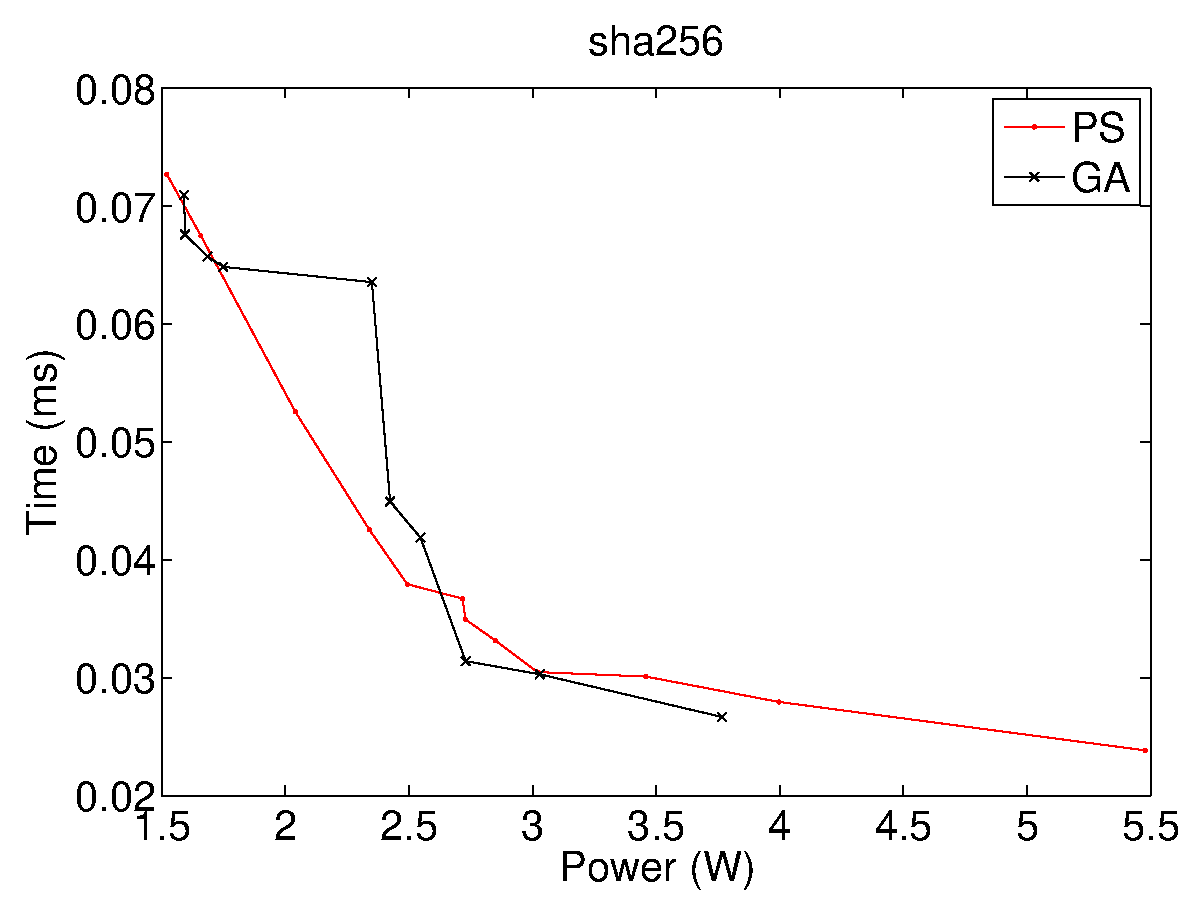
\includegraphics[width=0.30\textwidth]{pictures/sha_100.eps} &
%    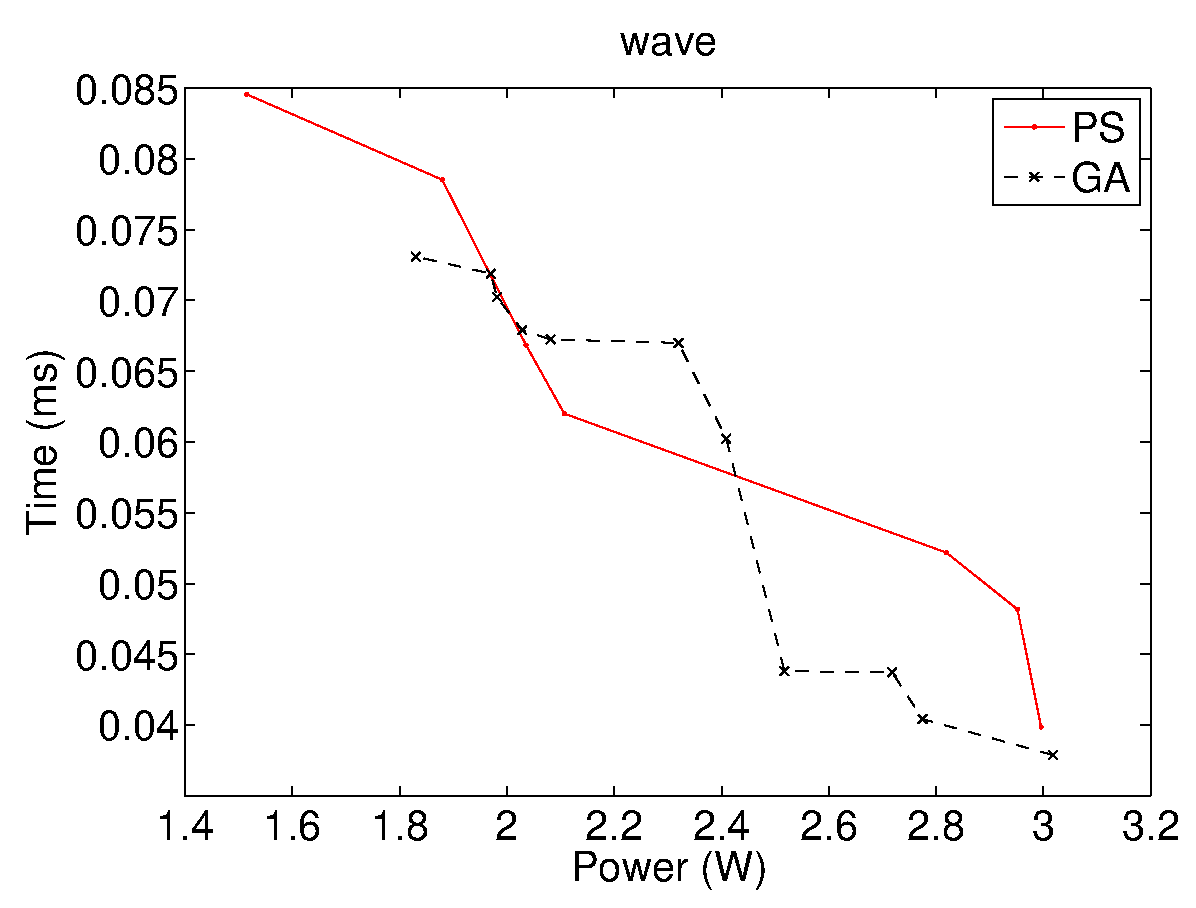
\includegraphics[width=0.30\textwidth]{pictures/wave_100.eps} 
%  \end{tabular}
%  \caption{Pareto fronts found by PS and GA for a fixed budget of 100 configurations.}
%  \label{fig:pareto_fronts_100}
%\end{table}
%
%\begin{table}
%  \centering
%  \begin{tabular}{ccc}
%    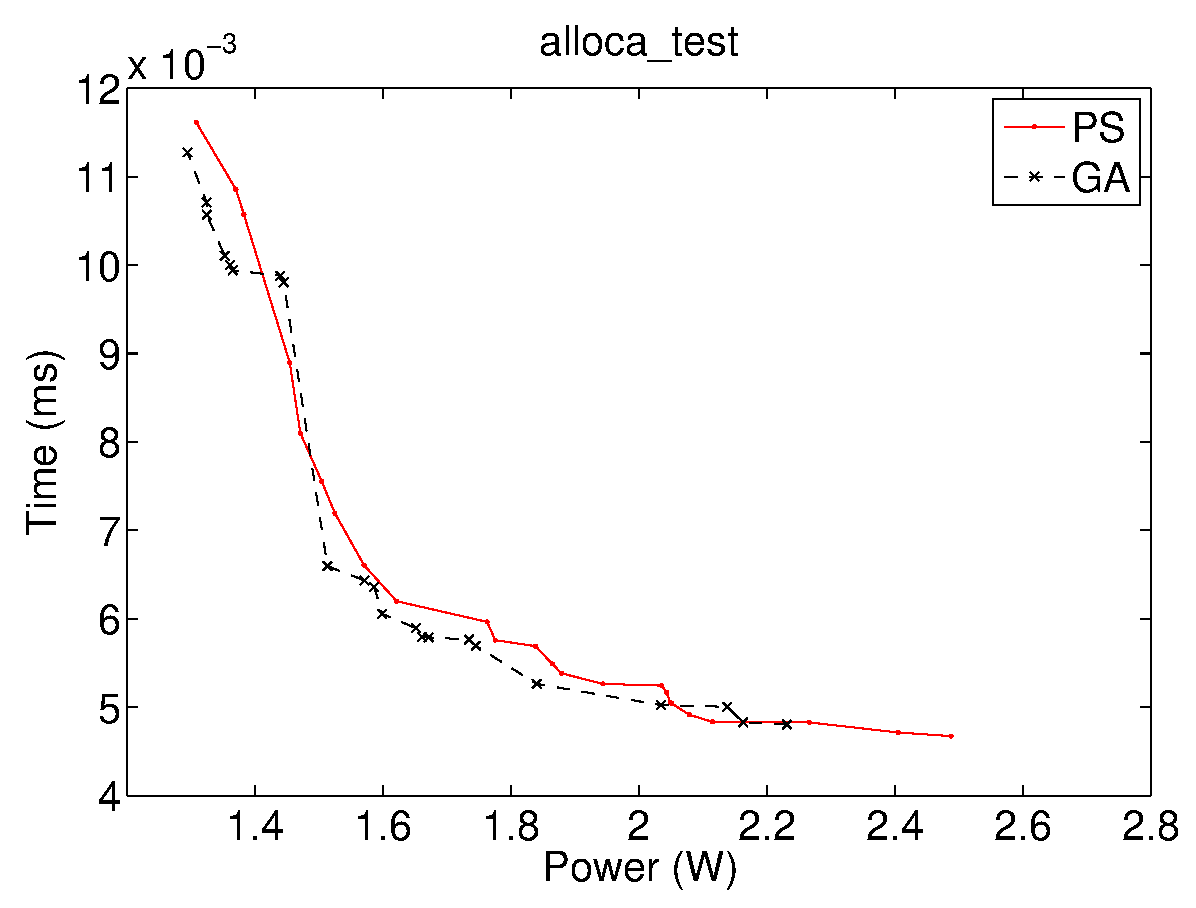
\includegraphics[width=0.30\textwidth]{pictures/alloca_500.eps} &
%    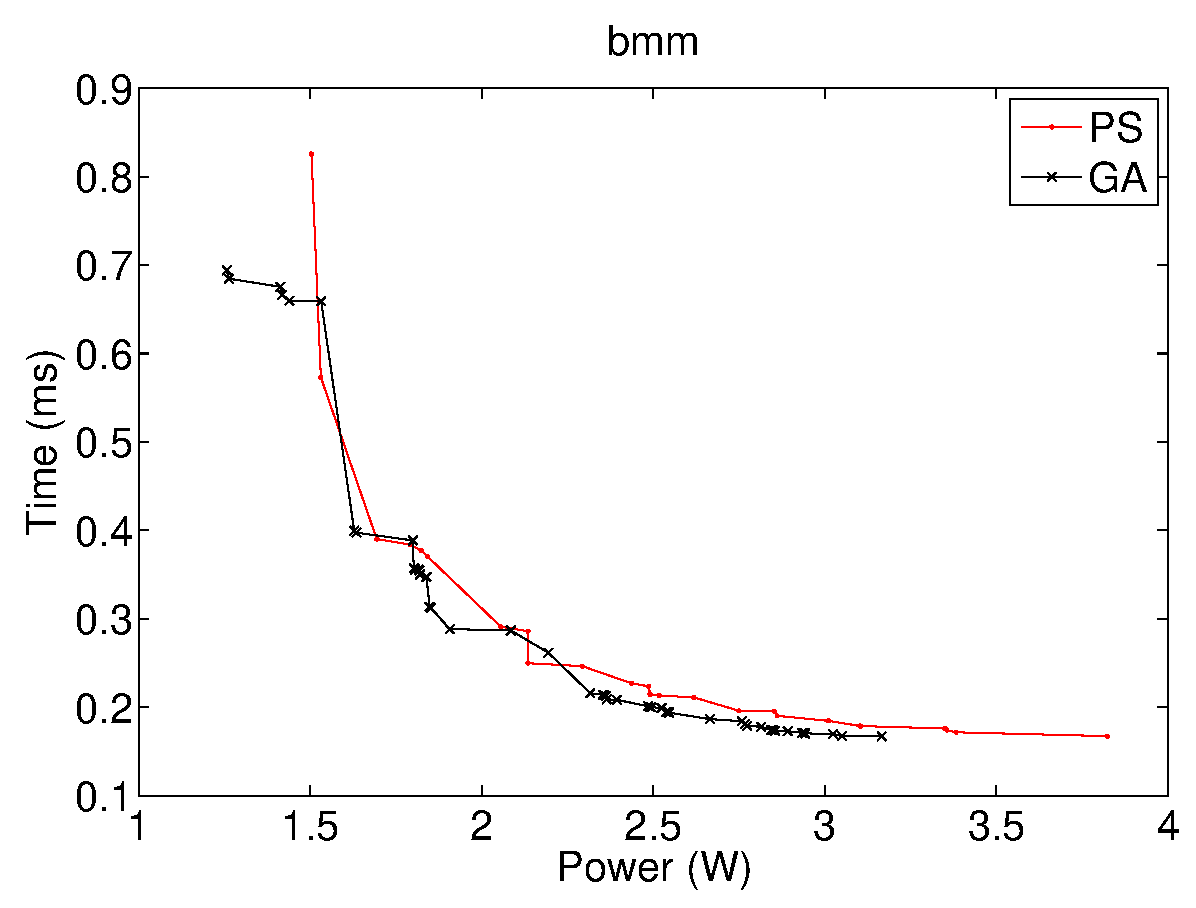
\includegraphics[width=0.30\textwidth]{pictures/bmm_500.eps} & 
%    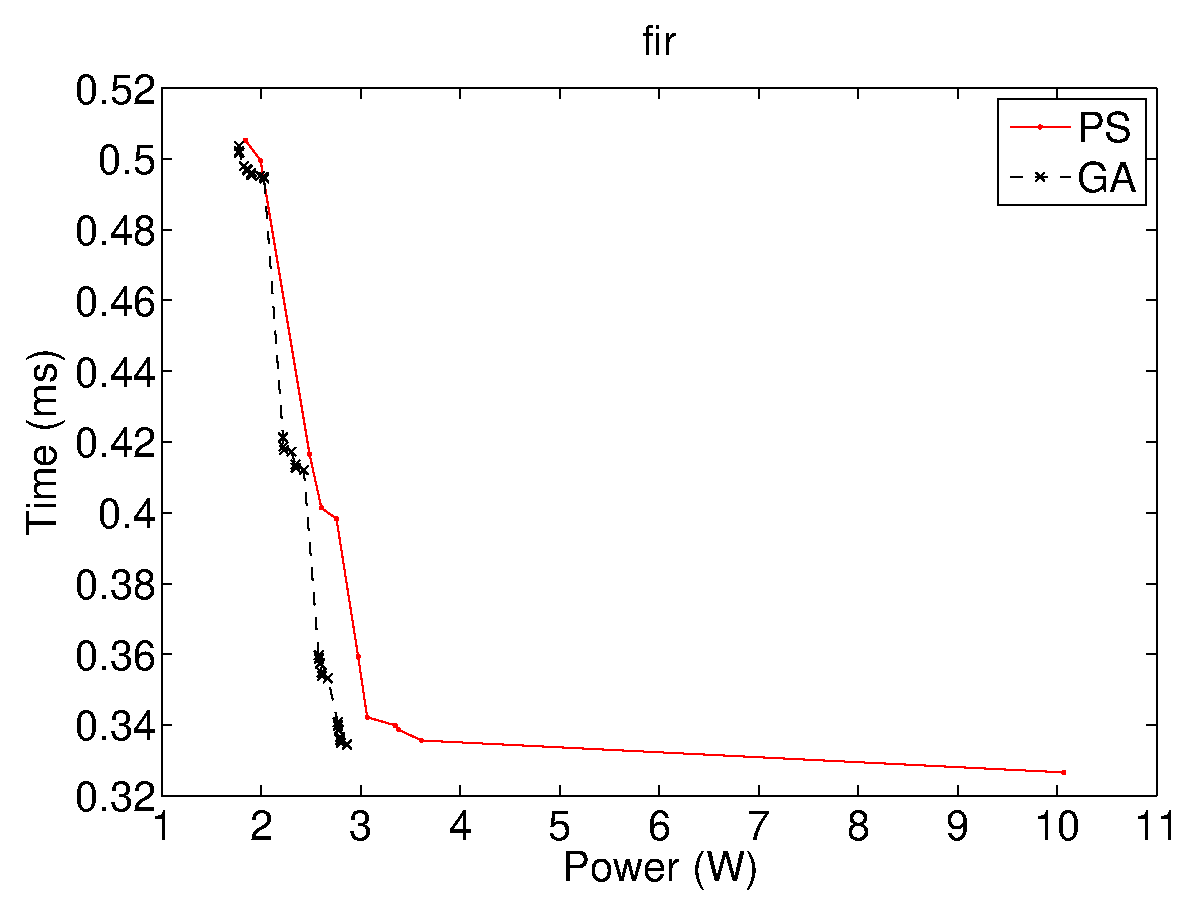
\includegraphics[width=0.30\textwidth]{pictures/fir_int500.eps} \\
%    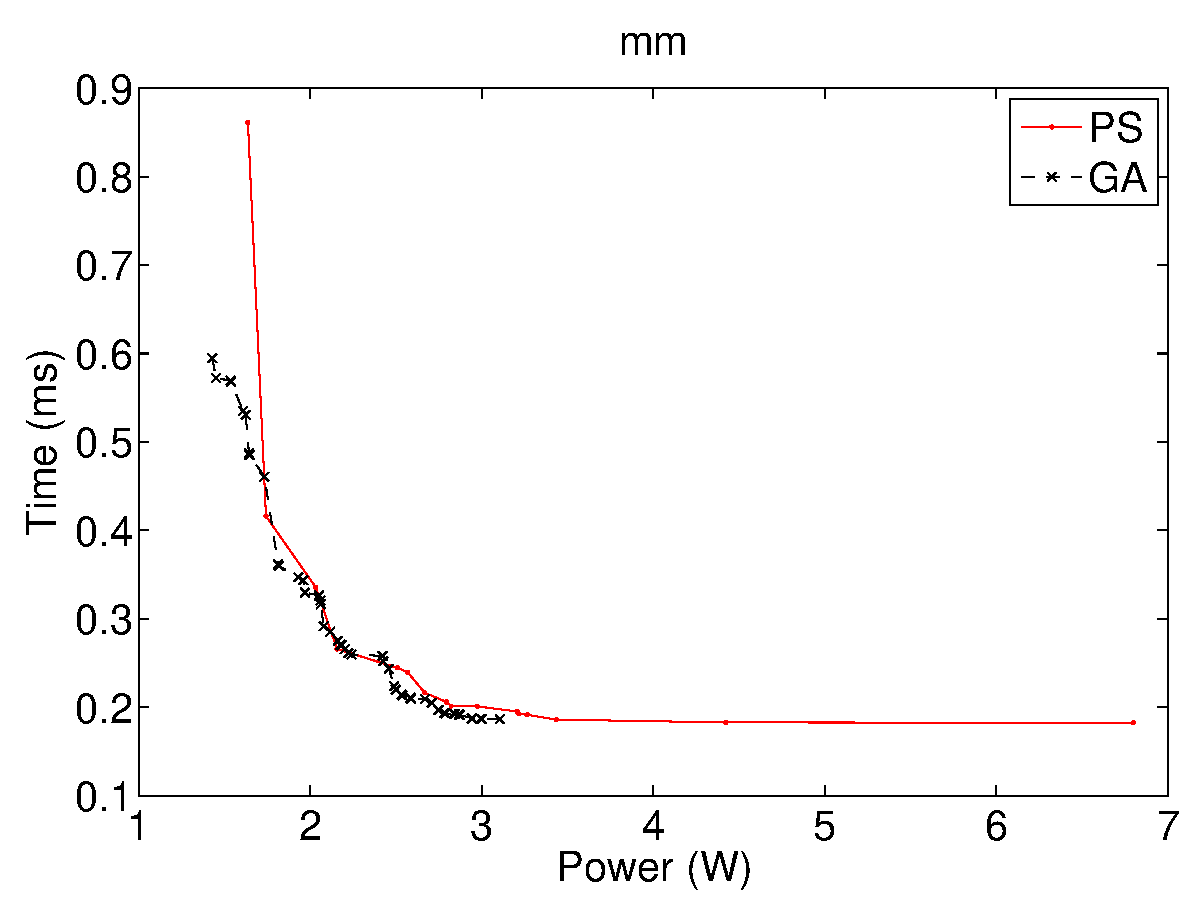
\includegraphics[width=0.30\textwidth]{pictures/mm_500.eps} &
%    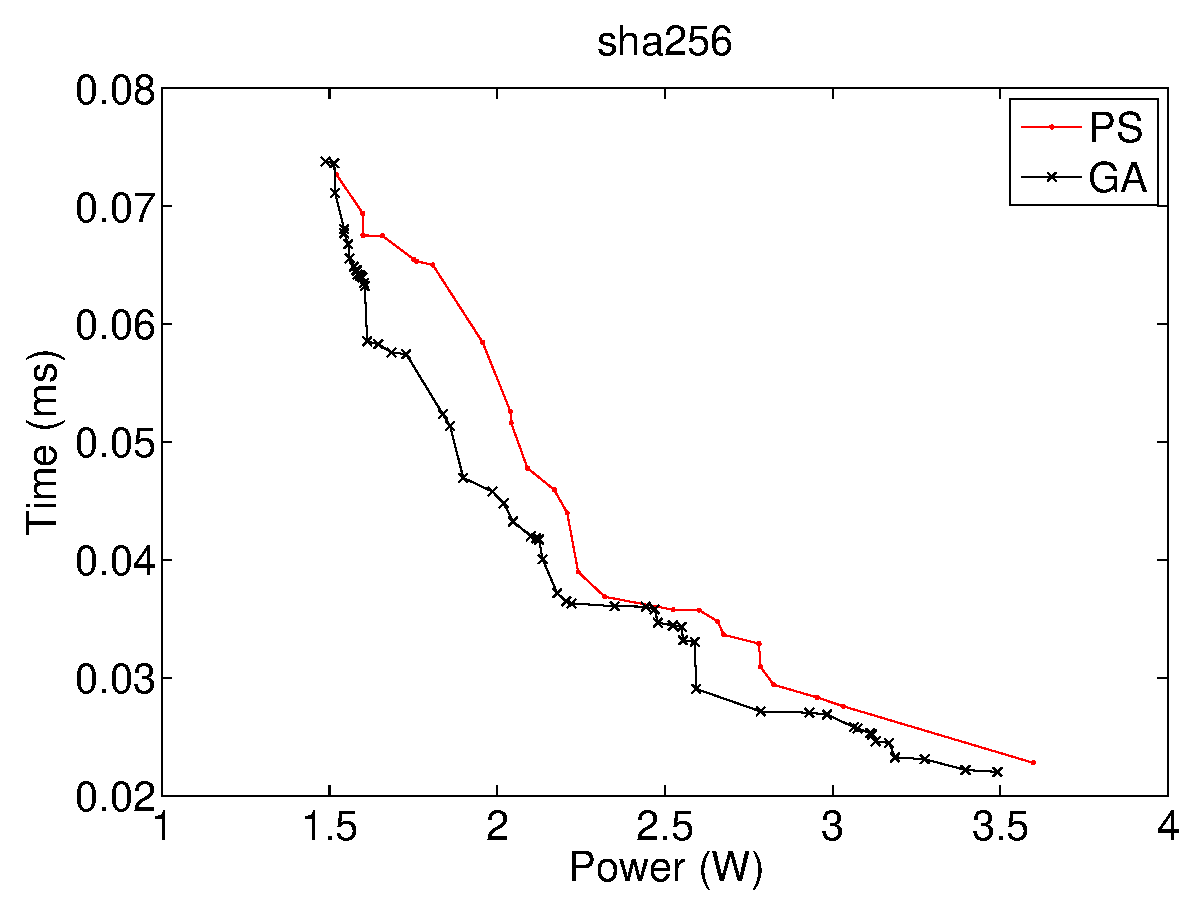
\includegraphics[width=0.30\textwidth]{pictures/sha_500.eps} &
%    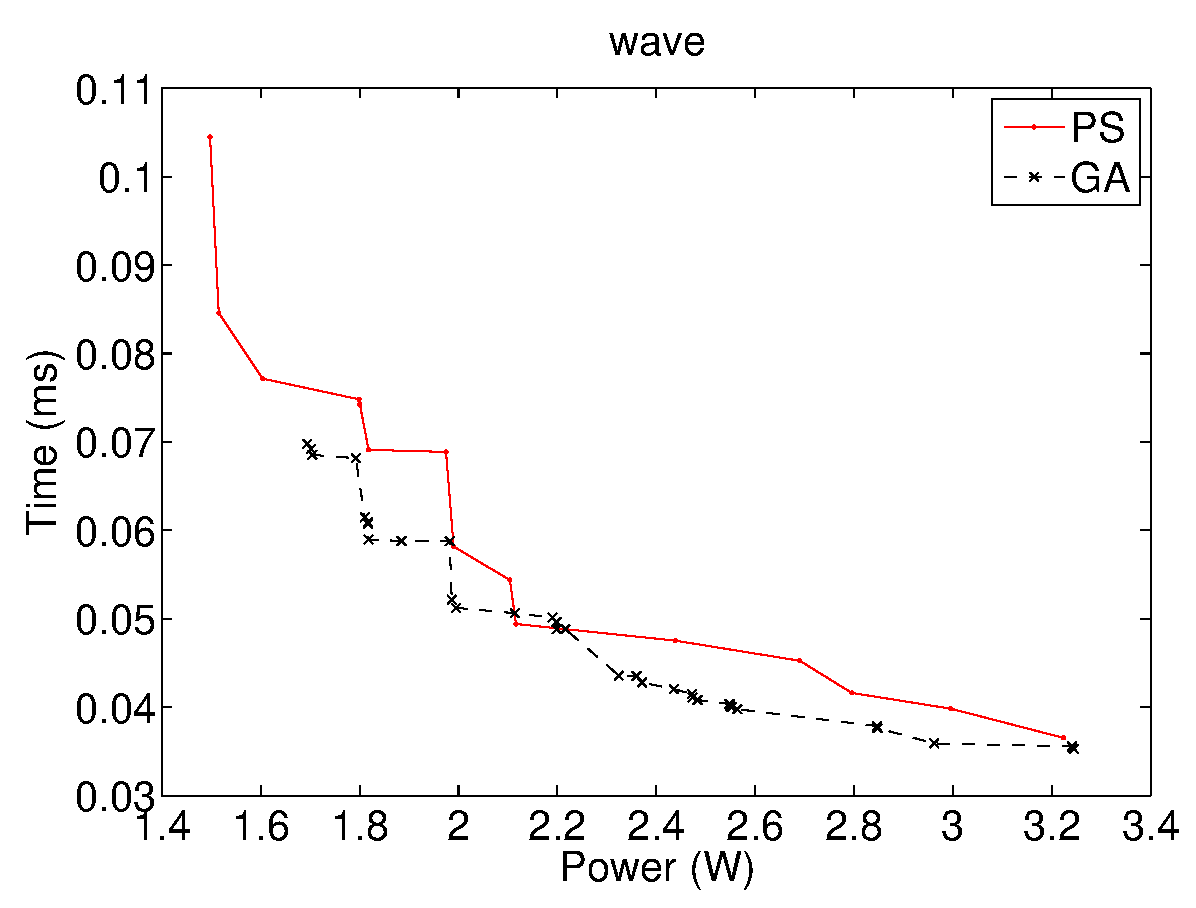
\includegraphics[width=0.30\textwidth]{pictures/wave_500.eps} 
%  \end{tabular}
%  \caption{Pareto fronts found by PS and GA for a fixed budget of 500 configurations.}
%  \label{fig:pareto_fronts_500}
%\end{table}

\begin{figure}
  \figLC{pareto_fronts_100}{Pareto fronts found by PS and GA for a fixed budget of 100 configurations. \comment{AA: nelle due figure centrali la linea di GA e' continua, mentre in tutte le altre figure e' tratteggiata. Il revisore ci chiede di uniformare. Non so come riottenere le figure. Potresti pensarci tu?}}
  \begin{center}
    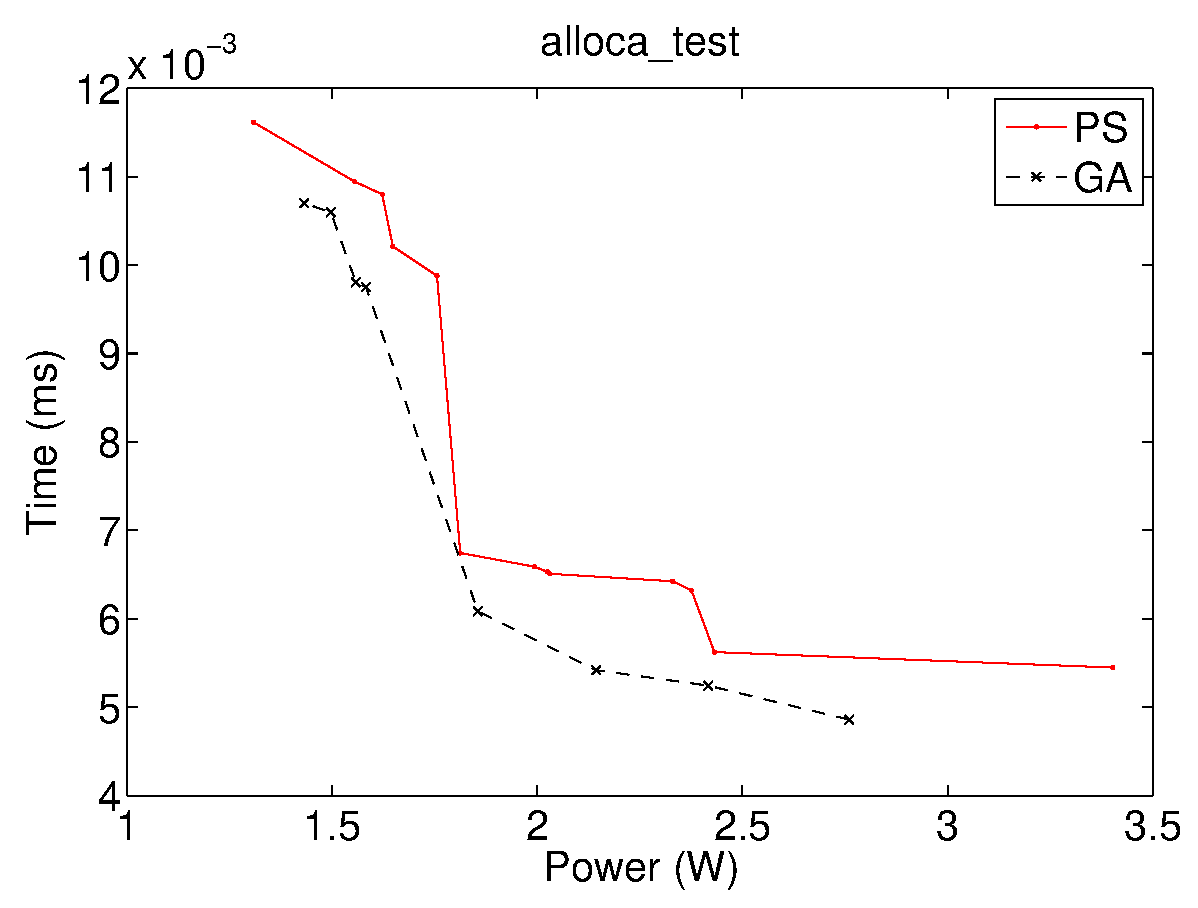
\includegraphics[width=0.30\textwidth]{pictures/alloca_100.eps}
    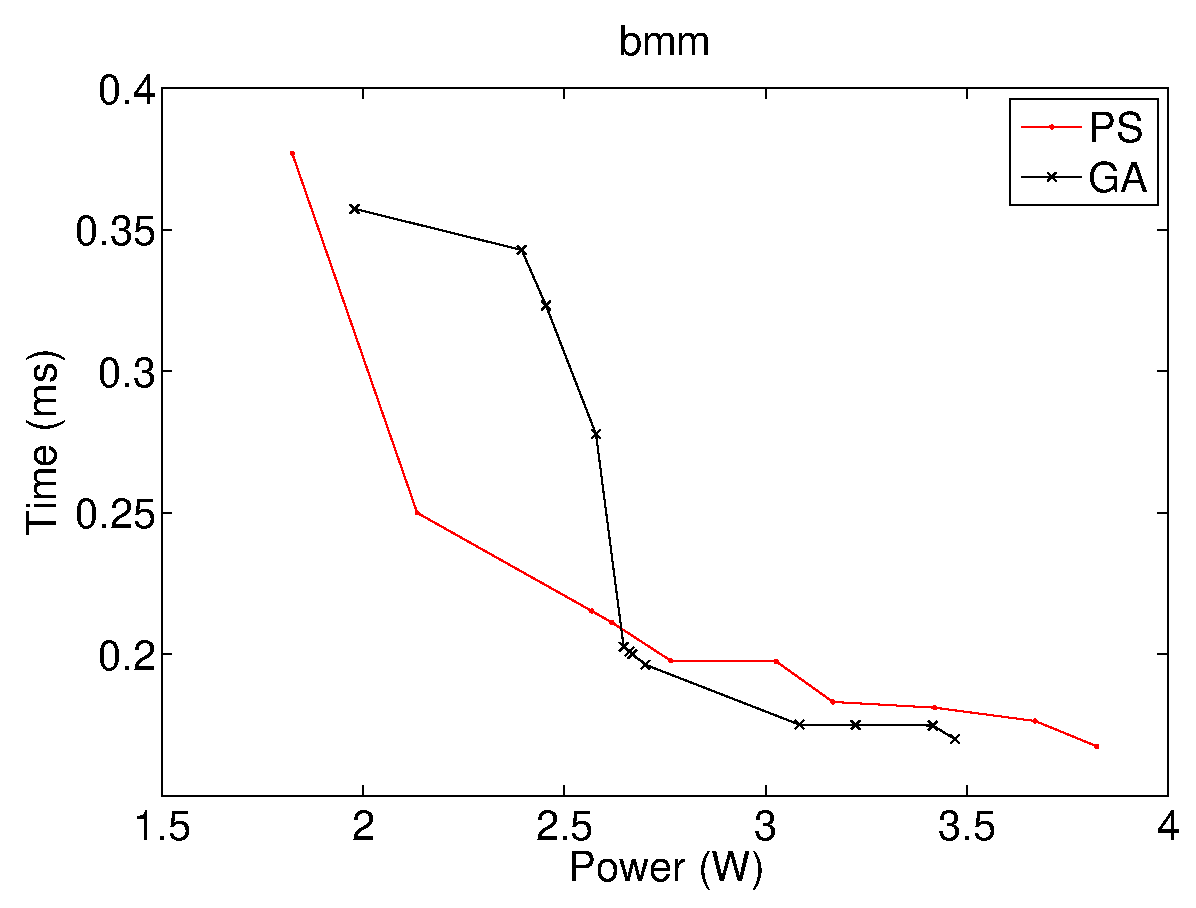
\includegraphics[width=0.30\textwidth]{pictures/bmm_100.eps}
    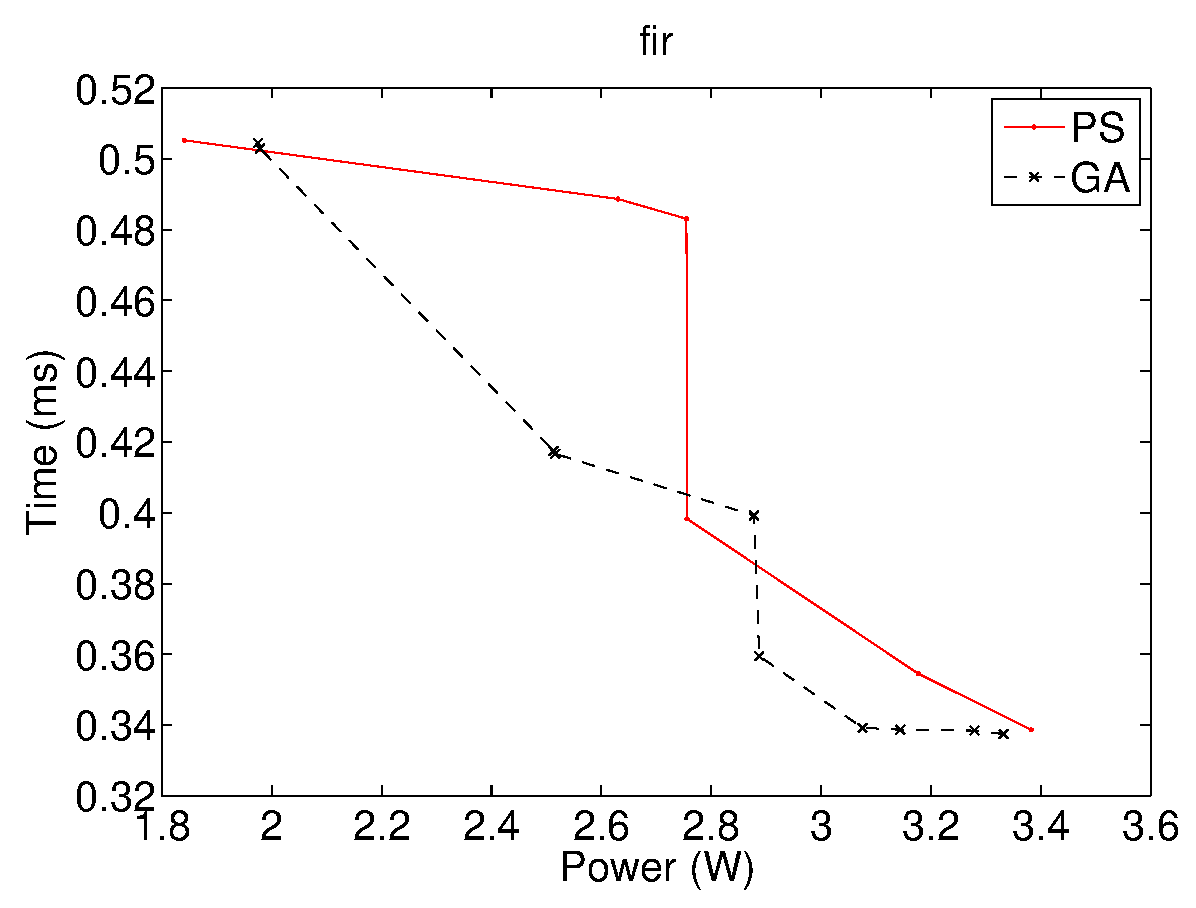
\includegraphics[width=0.30\textwidth]{pictures/fir_int100.eps}
    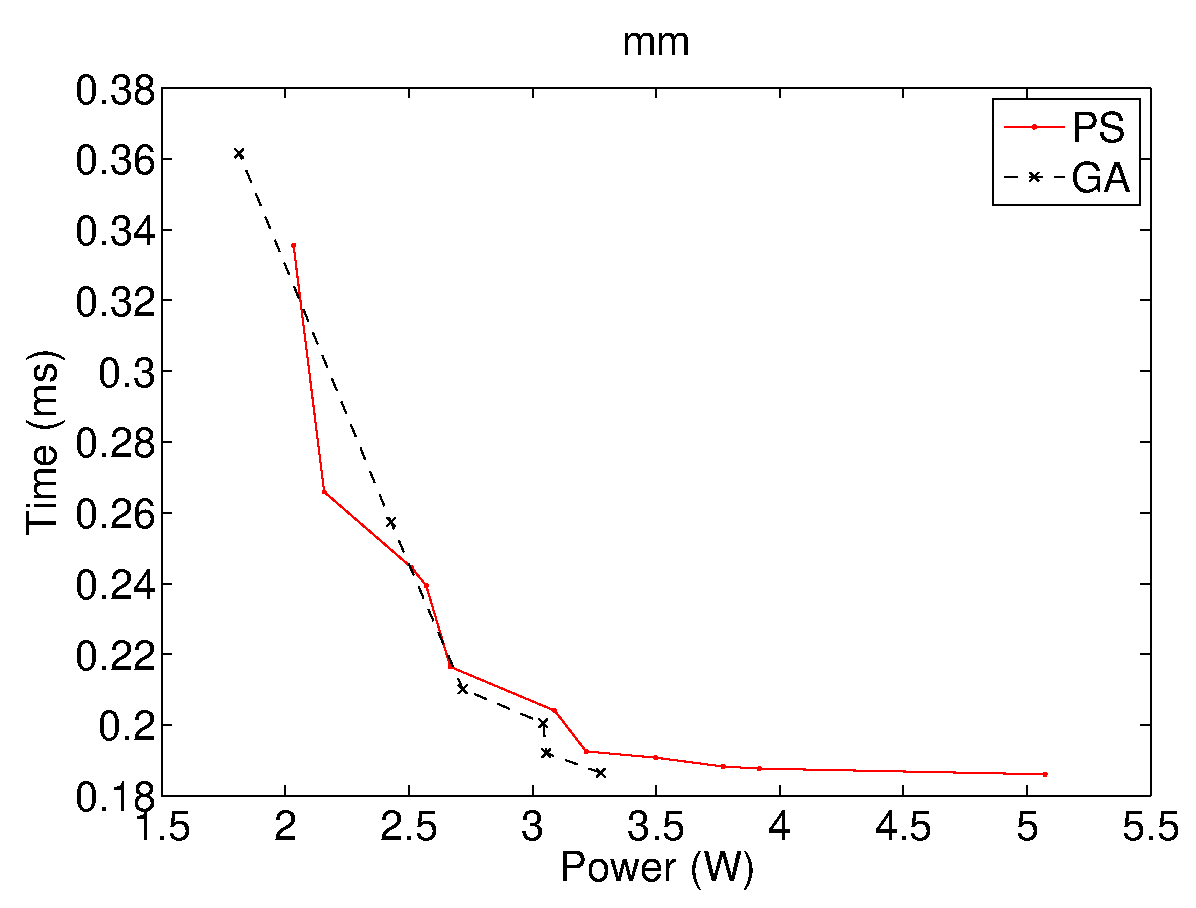
\includegraphics[width=0.30\textwidth]{pictures/mm_100.eps}
    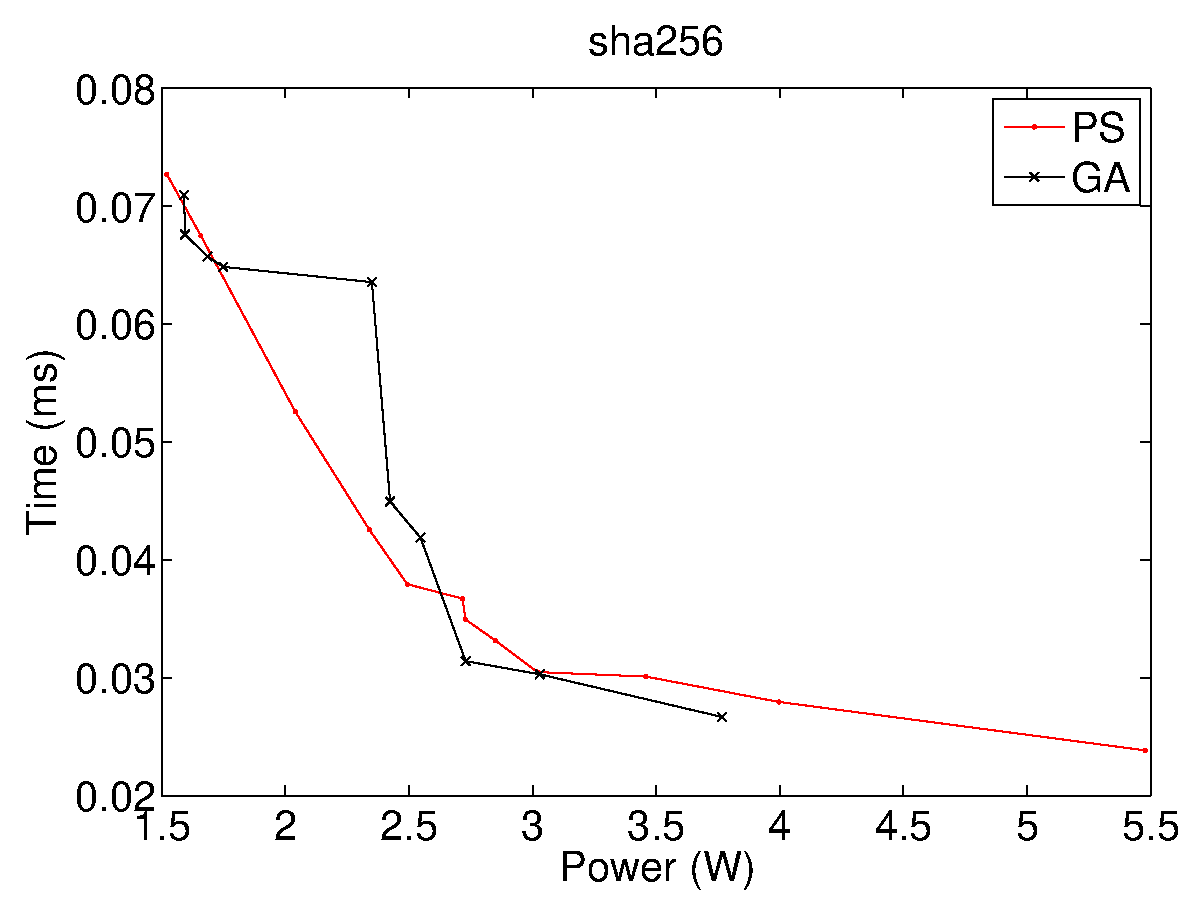
\includegraphics[width=0.30\textwidth]{pictures/sha_100.eps}
    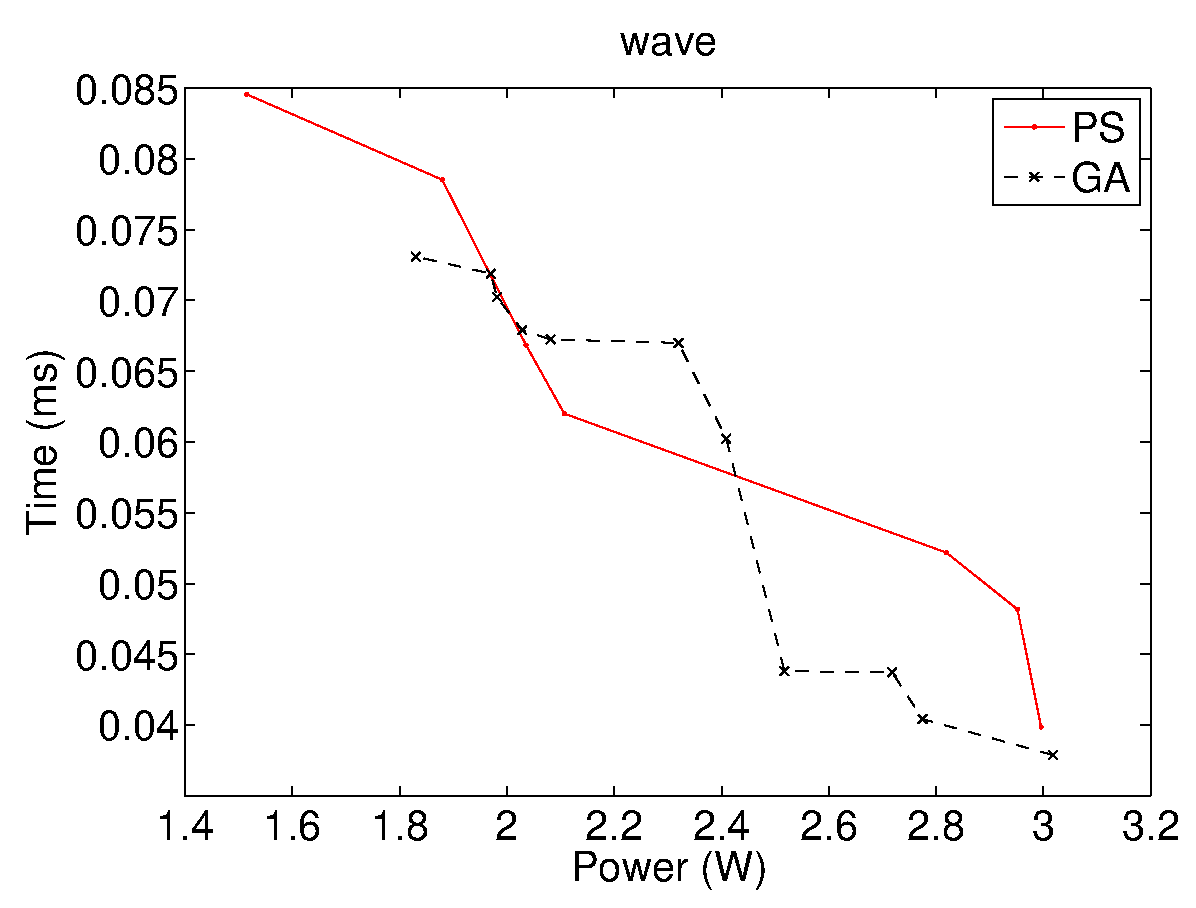
\includegraphics[width=0.30\textwidth]{pictures/wave_100.eps} 
  \end{center}
\end{figure}

\begin{figure}
  \figLC{pareto_fronts_500}{Pareto fronts found by PS and GA for a fixed budget of 500 configurations.\comment{AA: nelle due figure centrali la linea di GA e' continua, mentre in tutte le altre figure e' tratteggiata. Il revisore ci chiede di uniformare. Non so come riottenere le figure. Potresti pensarci tu?}}
  \begin{center}
    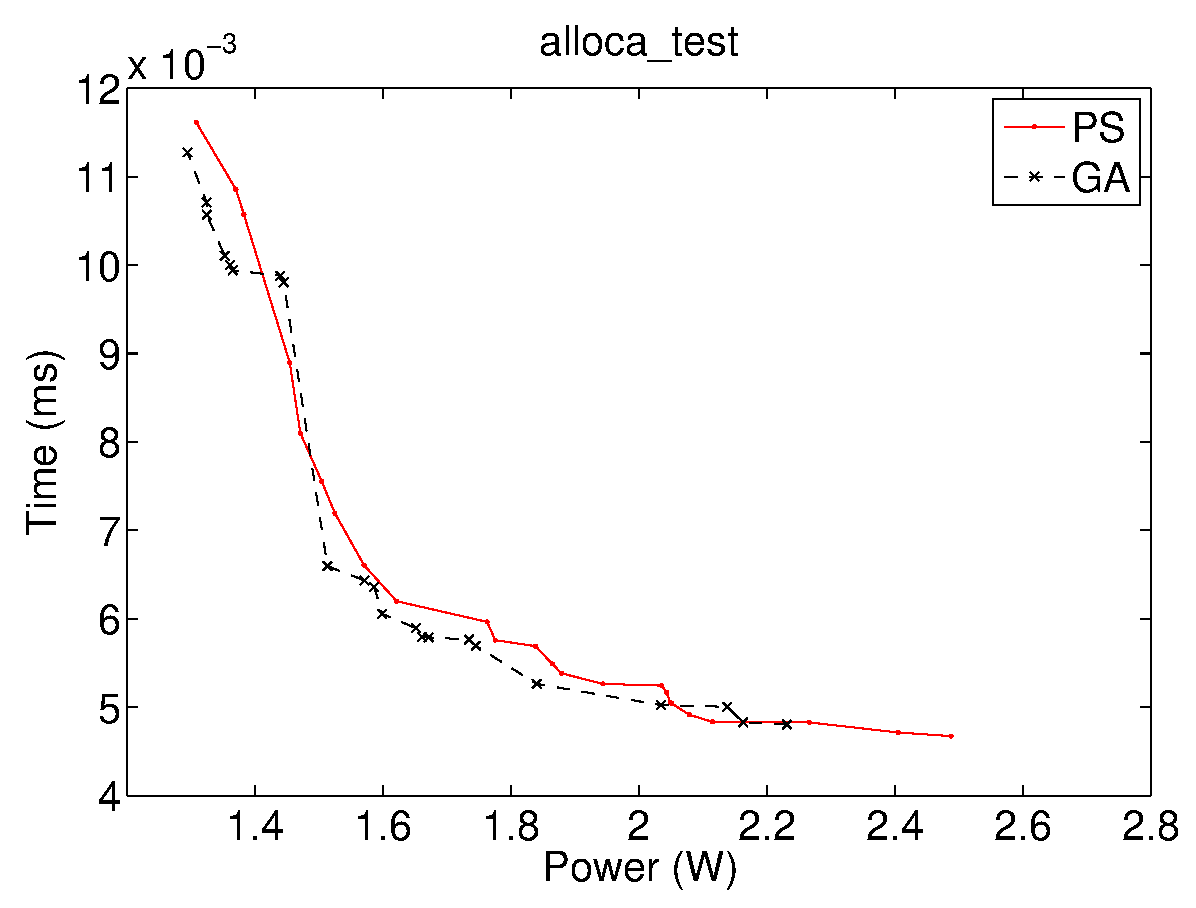
\includegraphics[width=0.30\textwidth]{pictures/alloca_500.eps}
    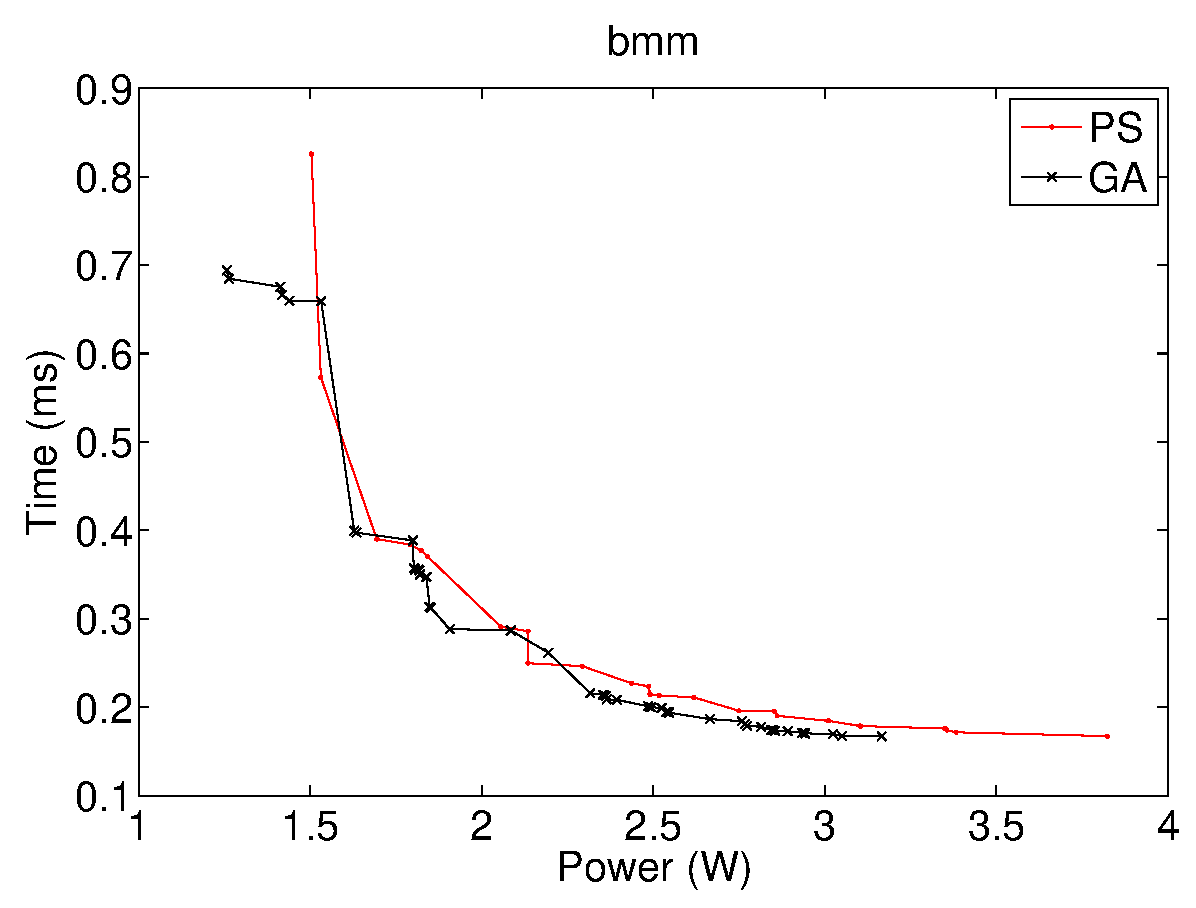
\includegraphics[width=0.30\textwidth]{pictures/bmm_500.eps}
    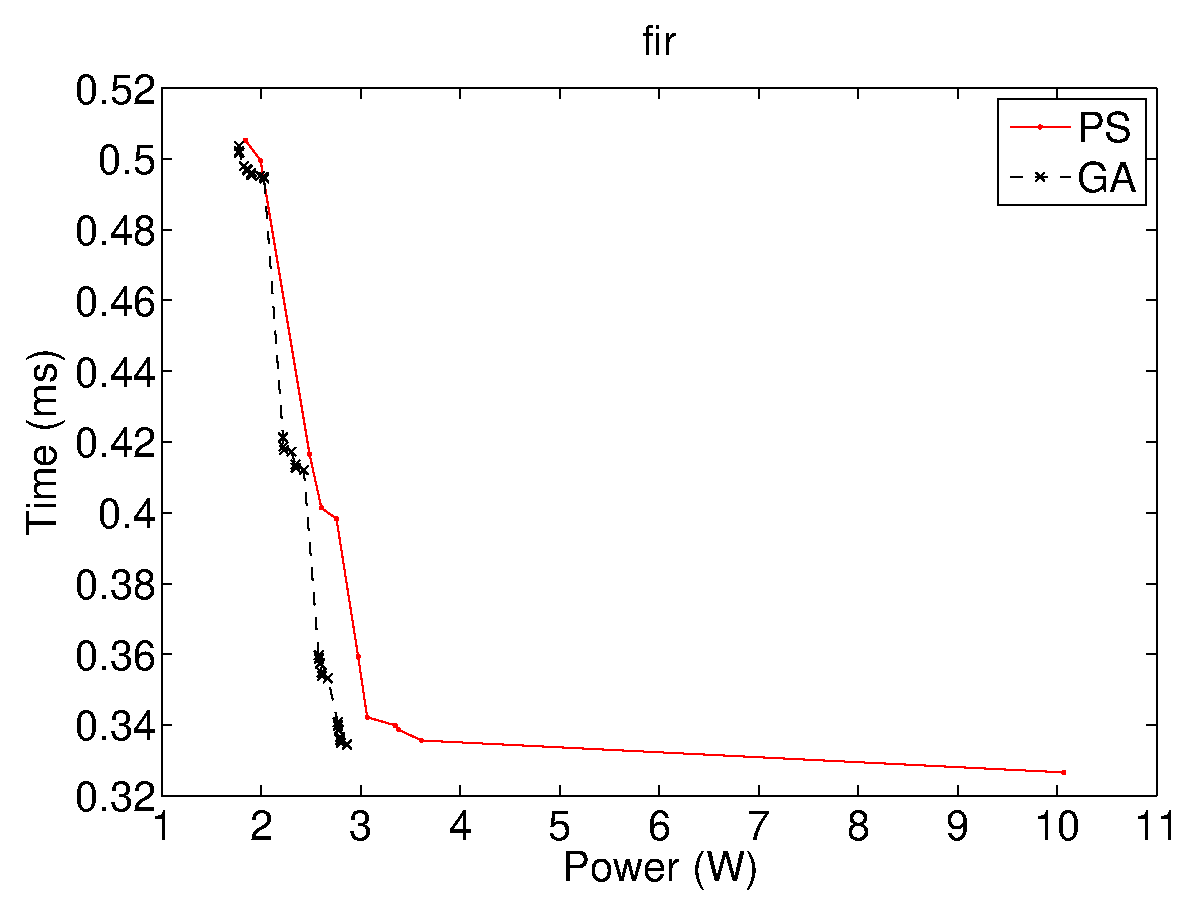
\includegraphics[width=0.30\textwidth]{pictures/fir_int500.eps}
    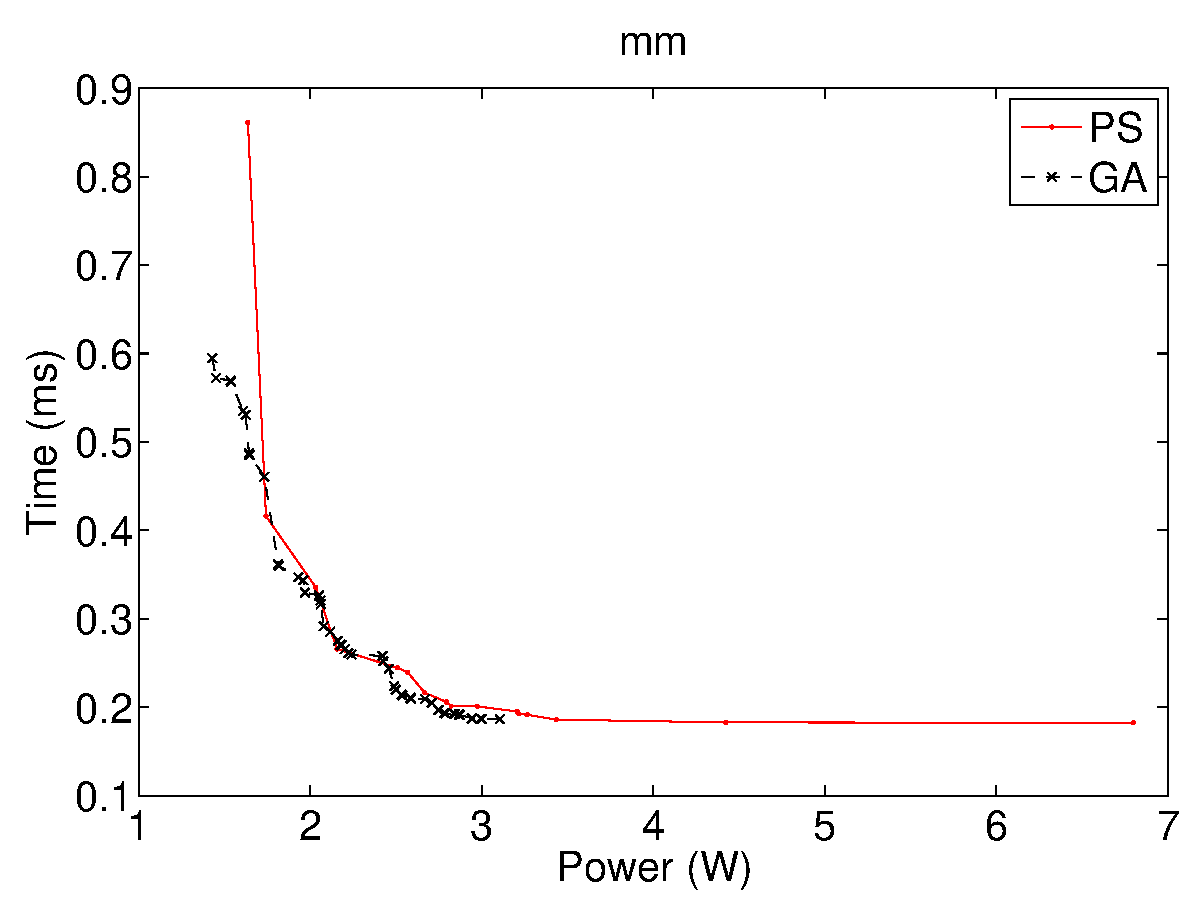
\includegraphics[width=0.30\textwidth]{pictures/mm_500.eps}
    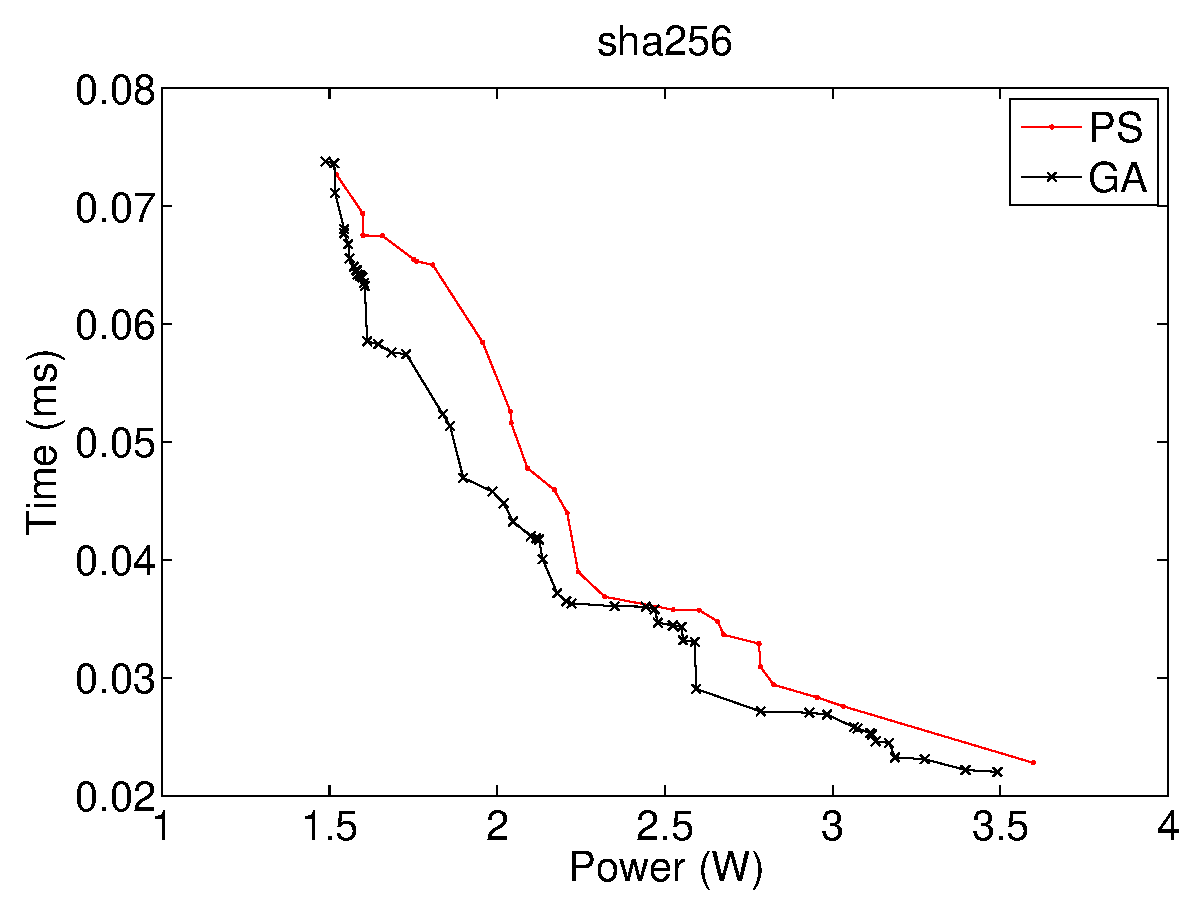
\includegraphics[width=0.30\textwidth]{pictures/sha_500.eps}
    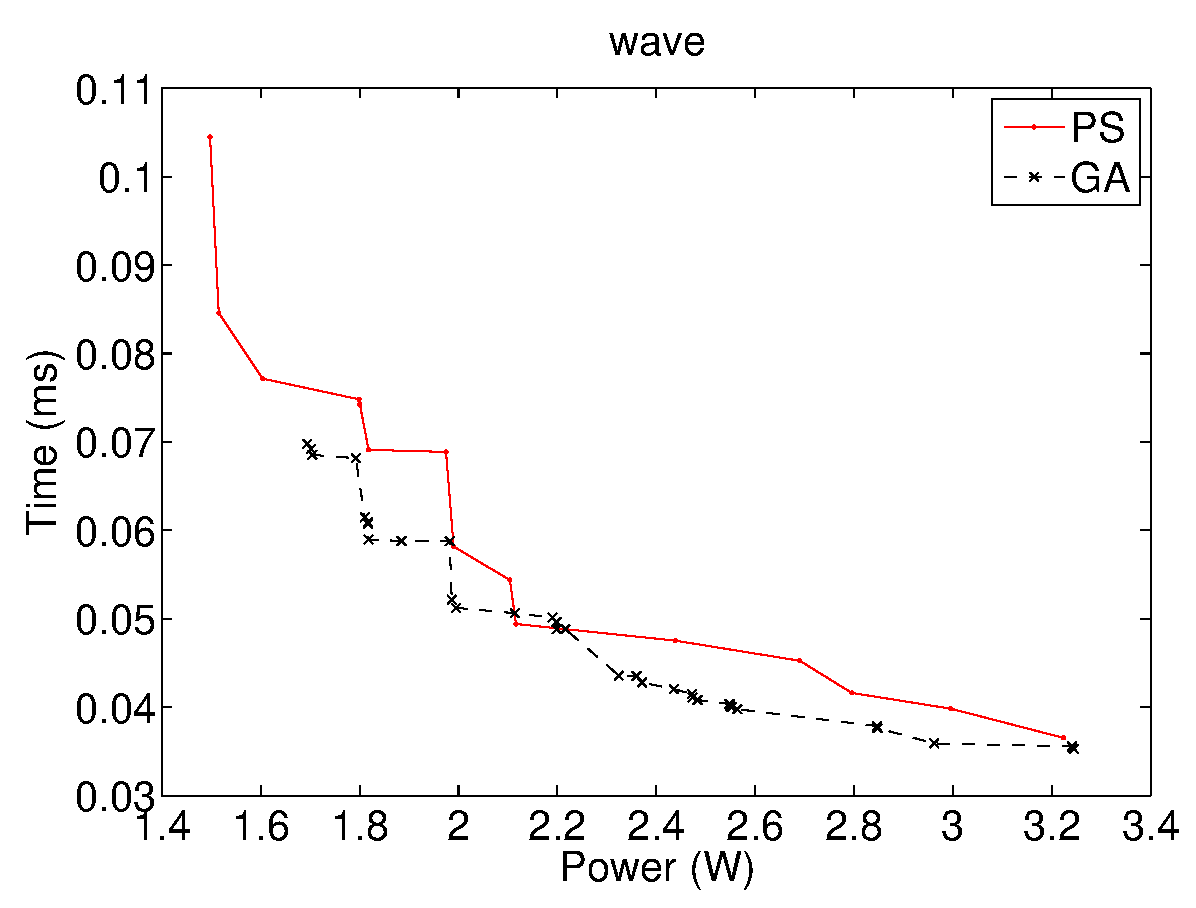
\includegraphics[width=0.30\textwidth]{pictures/wave_500.eps} 
  \end{center}
\end{figure}
Low budget Pareto sets are shown in \figR{pareto_fronts_100}. With a so small number of
configuration being investigated the two sets are often overlapping,
being also strongly dependent upon the application being considered.
These results are obtained in about 5 eras and demonstrate that with a so limited budget PS can compete with
genetic approach while even discovering very different Pareto fronts. 
Considering the extended simulation budget as depicted in
\figR{pareto_fronts_500}, we can qualitatively observe that
even if PS does not strictly outperforms genetic in terms of dominance, it shows in
some cases largely Pareto in terms of extension. We can intuitively
relate this to the ``novelty-based'' score system, so that instead of
focusing on getting better points inside a given range it tries to
enlarge the range itself, resulting in less dense but more extended
Paretos. Of course we cannot classify this different behaviour as
``better'' or ``worse'' as compared to the genetic one, it depends on
various design factors such as desired results granularity, prefixed objective
range constraints, estimated error of the models used etc.


A comparison between the variation ranges of both power dissipation
and execution time, obtained by PS and GA for different benchmarks is
shown in \figR{dispersion}(a) and (b) respectively.  As it can
be observed, the PS exploration provides solutions which fall on a
range that is, on average, wider than the one provided by a GA
exploration for power dissipation and execution time, respectively.
%\begin{table}
%  \centering
%  \begin{tabular}{c}
%    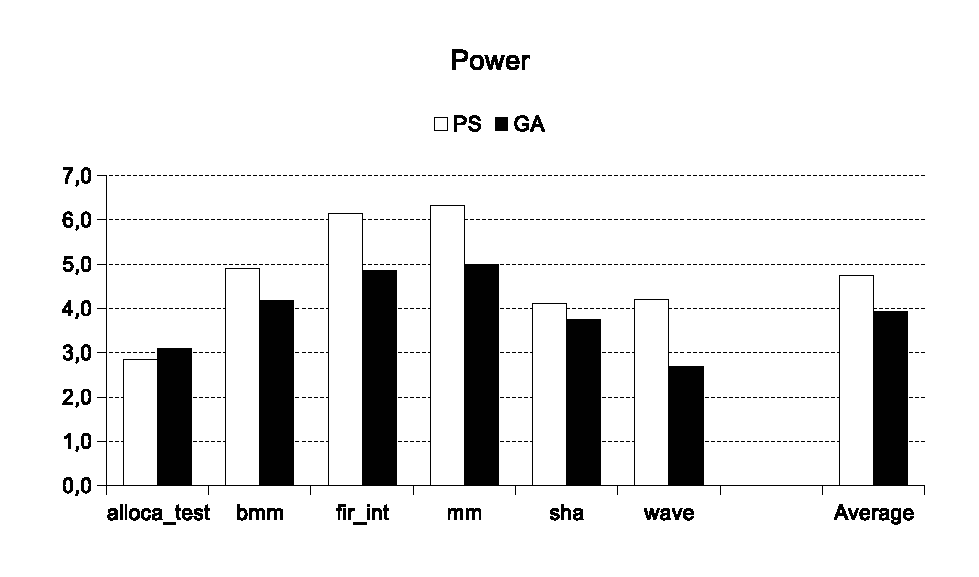
\includegraphics[width=0.7\textwidth]{pictures/variation_power.eps} \\
%    (a) \\
%    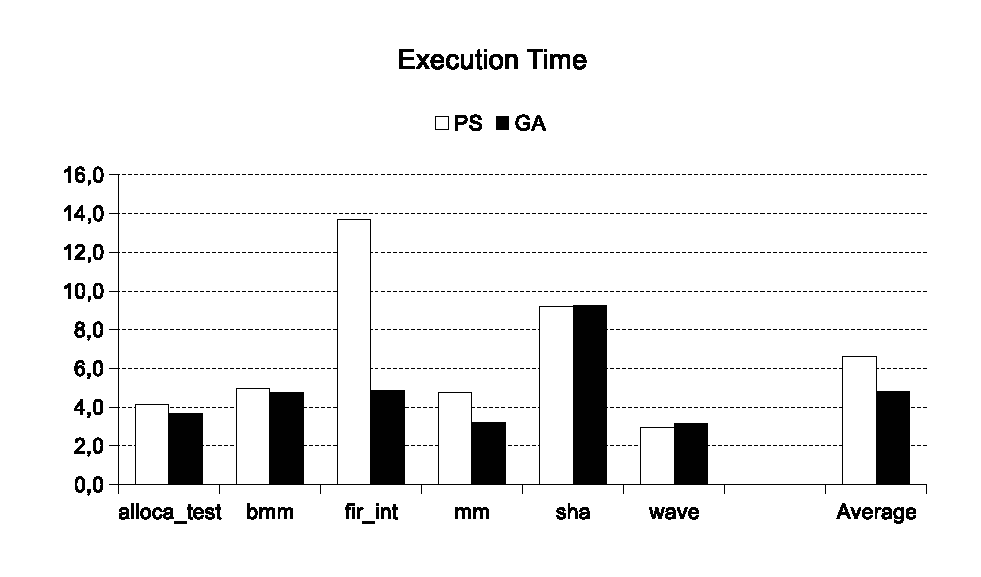
\includegraphics[width=0.7\textwidth]{pictures/variation_etime.eps} \\
%    (b) \\
%    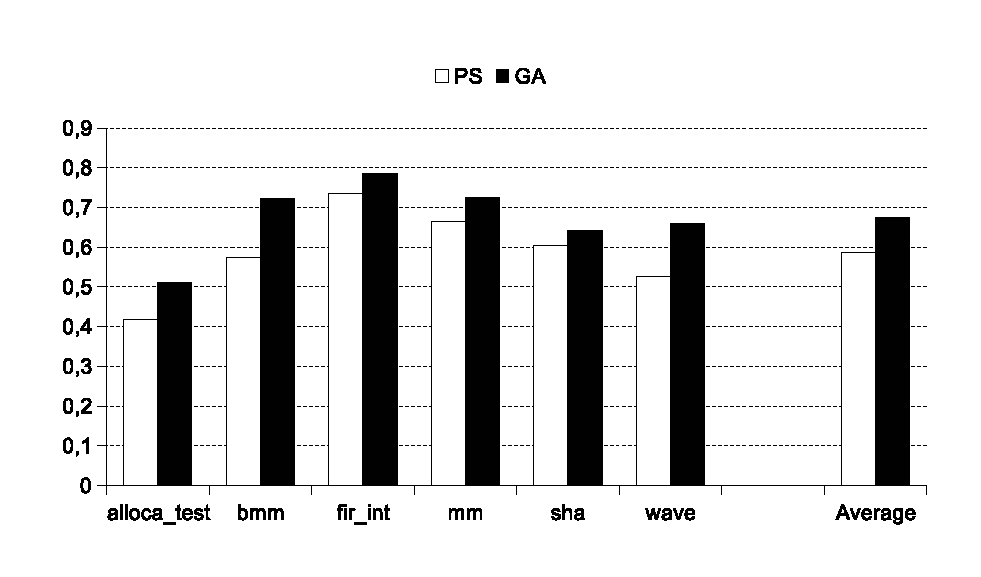
\includegraphics[width=0.7\textwidth]{pictures/dispersion.eps} \\
%    (c) 
%  \end{tabular}
%  \caption{(a)(b) Variation range obtained by PS and GA for different benchmarks
%  and average dispersion absolute dispersion (c)}
%  \label{fig:dispersion}
%\end{table}

\begin{figure}
  \figLC{dispersion}{(a)(b) Variation range obtained by PS and GA for different benchmarks and average dispersion absolute dispersion (c). \comment{AA: manca il titolo nella figura (c)} }
  \begin{center}
    \subfigure[]{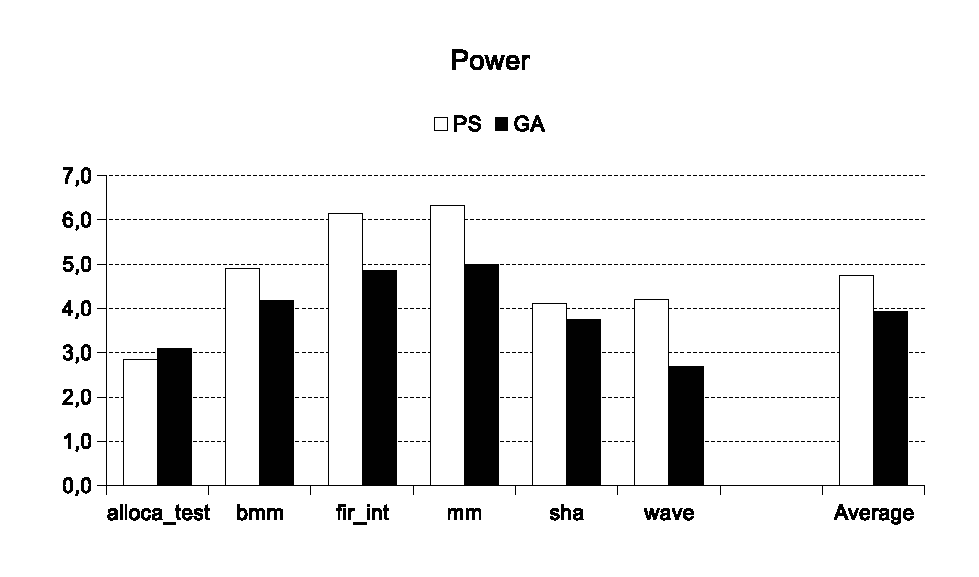
\includegraphics[width=0.7\textwidth]{pictures/variation_power.eps} }
    \subfigure[]{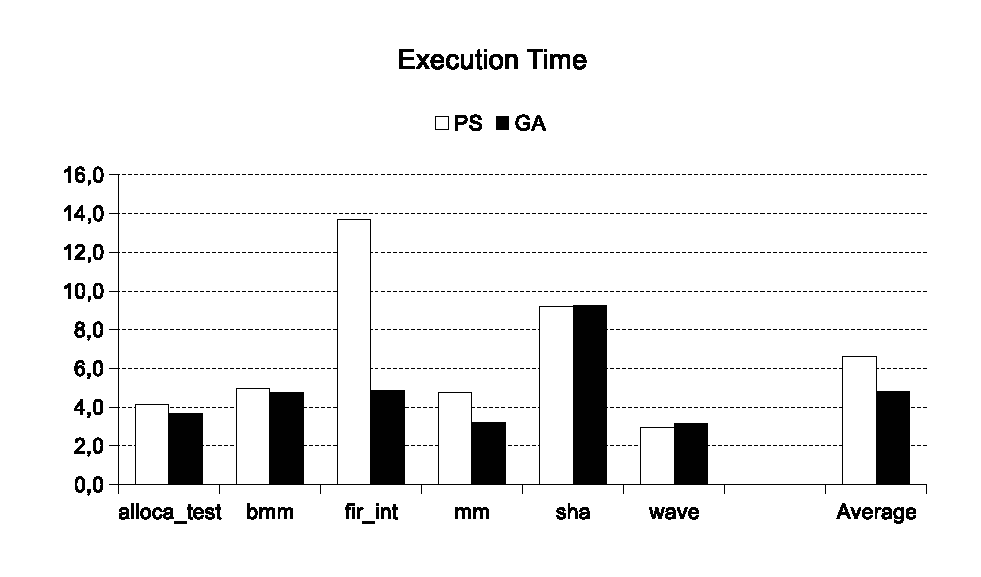
\includegraphics[width=0.7\textwidth]{pictures/variation_etime.eps} }
    \subfigure[]{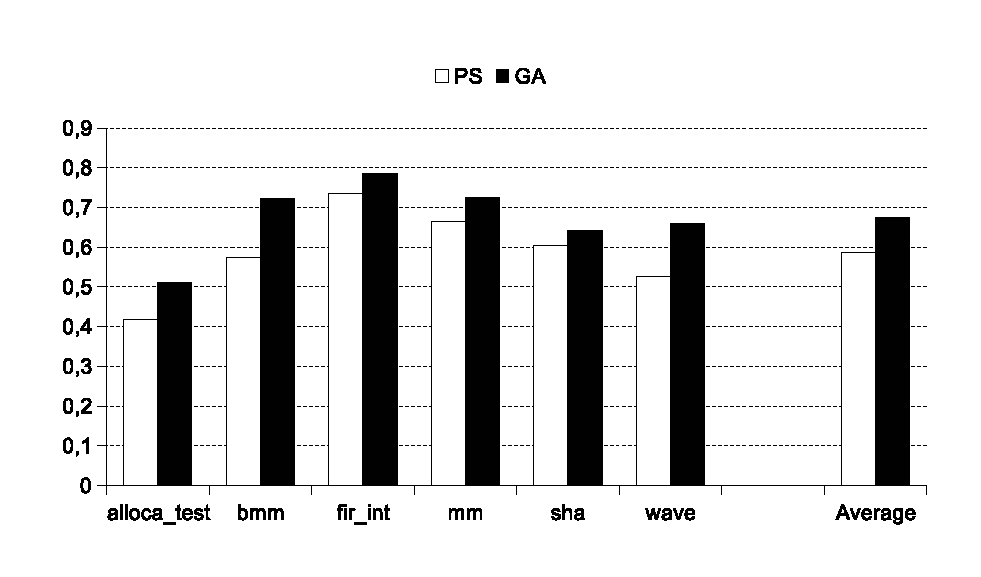
\includegraphics[width=0.7\textwidth]{pictures/dispersion.eps} }
  \end{center}
\end{figure}

\figR{dispersion}(c) shows the average normalised absolute
dispersion errors for different benchmarks for PS and GA
exploration. As it can be observed, GA shows a tendency in
discovering more uniformly dispersed points (i.e. higher values in the
chart). These results,
together with the variation ranges of \figR{dispersion}(a) and
(b) confirm the of density vs extension trade-offs
when comparing PS and GA approaches. Again, it
is worth pointing out how a definitive claim about the superiority of
the PS behaviour is strictly dependent on the design 
requirements and constraints, e.g. whether we need wide or dense
results. Nevertheless, the proposed algorithm introduces a new
perspective on the allocation of a simulations budget, paving the way for
the development of further strategies for addressing the problem of
multi-objective hardware/software design space exploration.

